\documentclass[11pt]{article}
\usepackage[utf8]{inputenc}
\usepackage[margin=1in]{geometry}
\usepackage{graphicx}
\usepackage{booktabs}
\usepackage{float}
\usepackage{siunitx}
\usepackage{amsmath}
\usepackage{hyperref}
\usepackage{xcolor}

\title{IEEE 118-Bus System Generator Analysis}
\author{Power System Analysis Report}
\date{\today}

\begin{document}
\maketitle

\section{Executive Summary}
This report presents a detailed analysis of the generator performance in the IEEE 118-bus system, comparing the original power flow solution with the OpenDSS implementation. The analysis focuses on both active and reactive power outputs, examining the accuracy of the implementation through statistical analysis and error assessment.

\section{Power Generation Analysis}

\subsection{Active Power Generation}
The active power generation analysis shows:
\begin{itemize}
    \item Mean generation: 81.01 MW
    \item Maximum generation: 607.00 MW (at Bus 89)
    \item Minimum generation: 0.00 MW
    \item 75\% of generators operate below 46.00 MW
\end{itemize}

\subsection{Reactive Power Generation}
The reactive power profile indicates:
\begin{itemize}
    \item Mean generation: 14.70 MVAR
    \item Maximum generation: 115.65 MVAR
    \item Minimum generation: -82.38 MVAR (absorption)
    \item Wide range of operation from absorbing to supplying reactive power
\end{itemize}

\section{Comparison Analysis}
\begin{figure}[H]
    \centering
    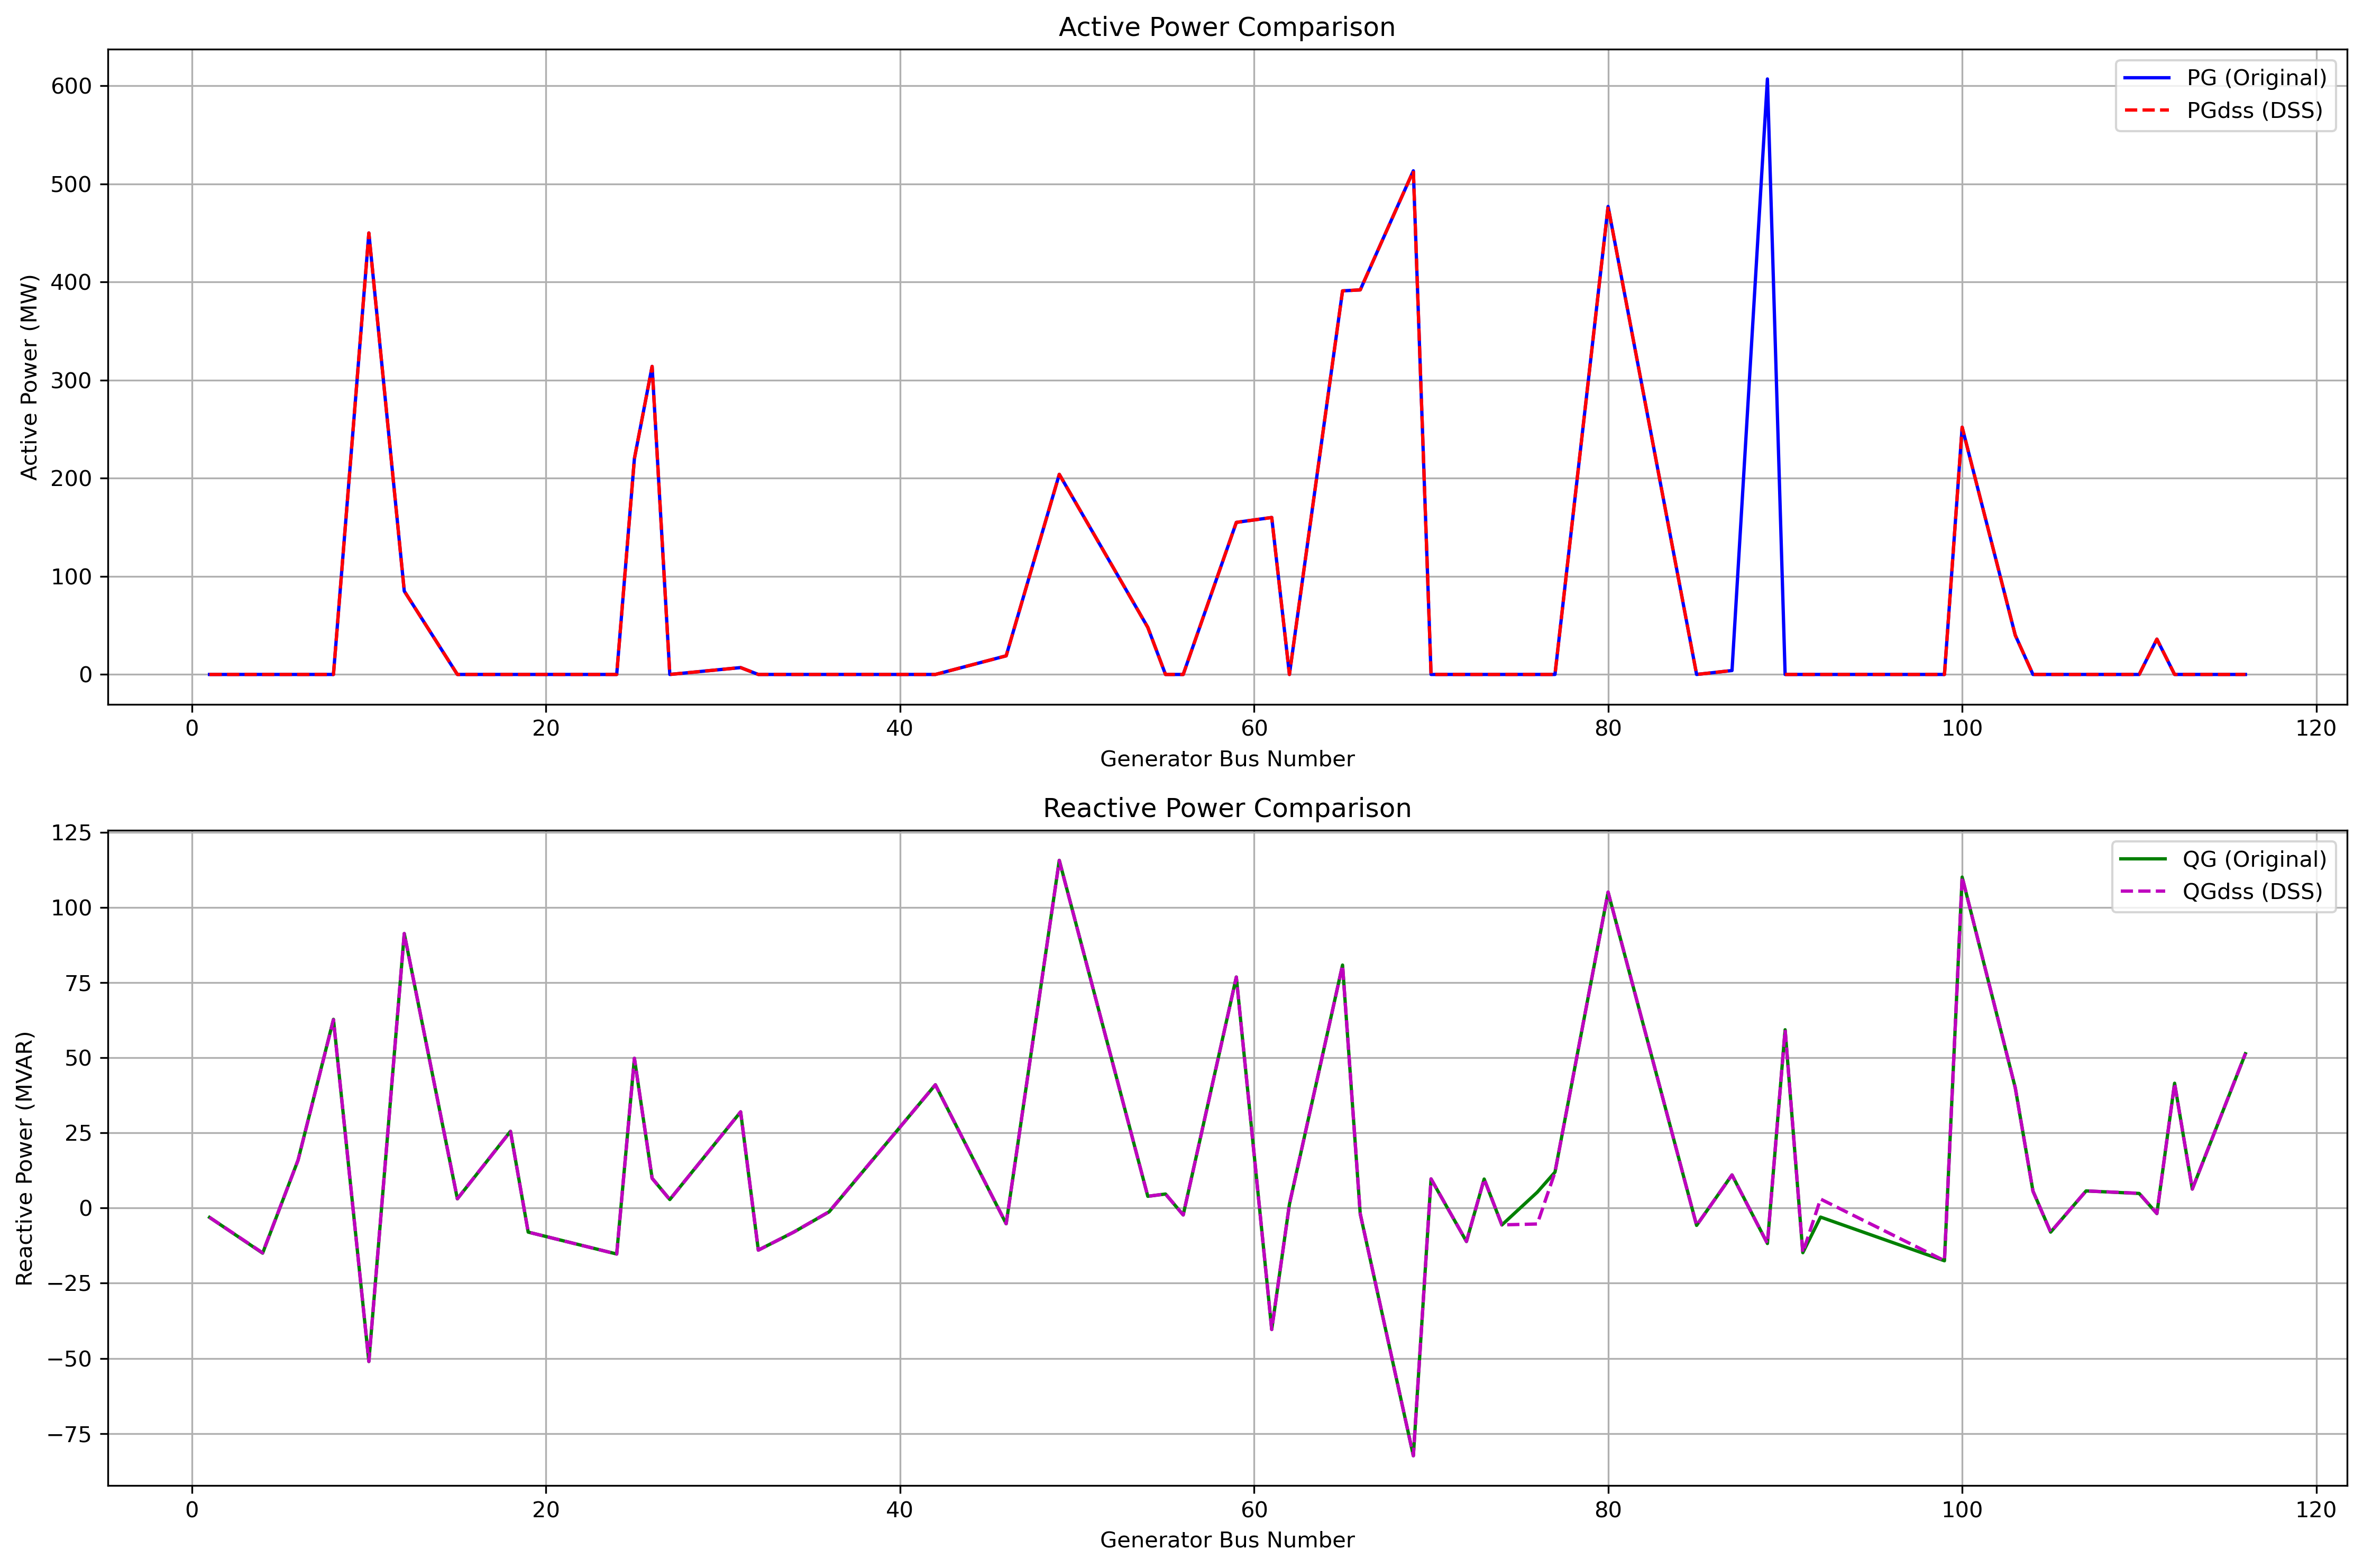
\includegraphics[width=\textwidth]{power_comparison.png}
    \caption{Comparison of Active and Reactive Power Generation}
    \label{fig:power_comparison}
\end{figure}

\section{Error Analysis}
\begin{figure}[H]
    \centering
    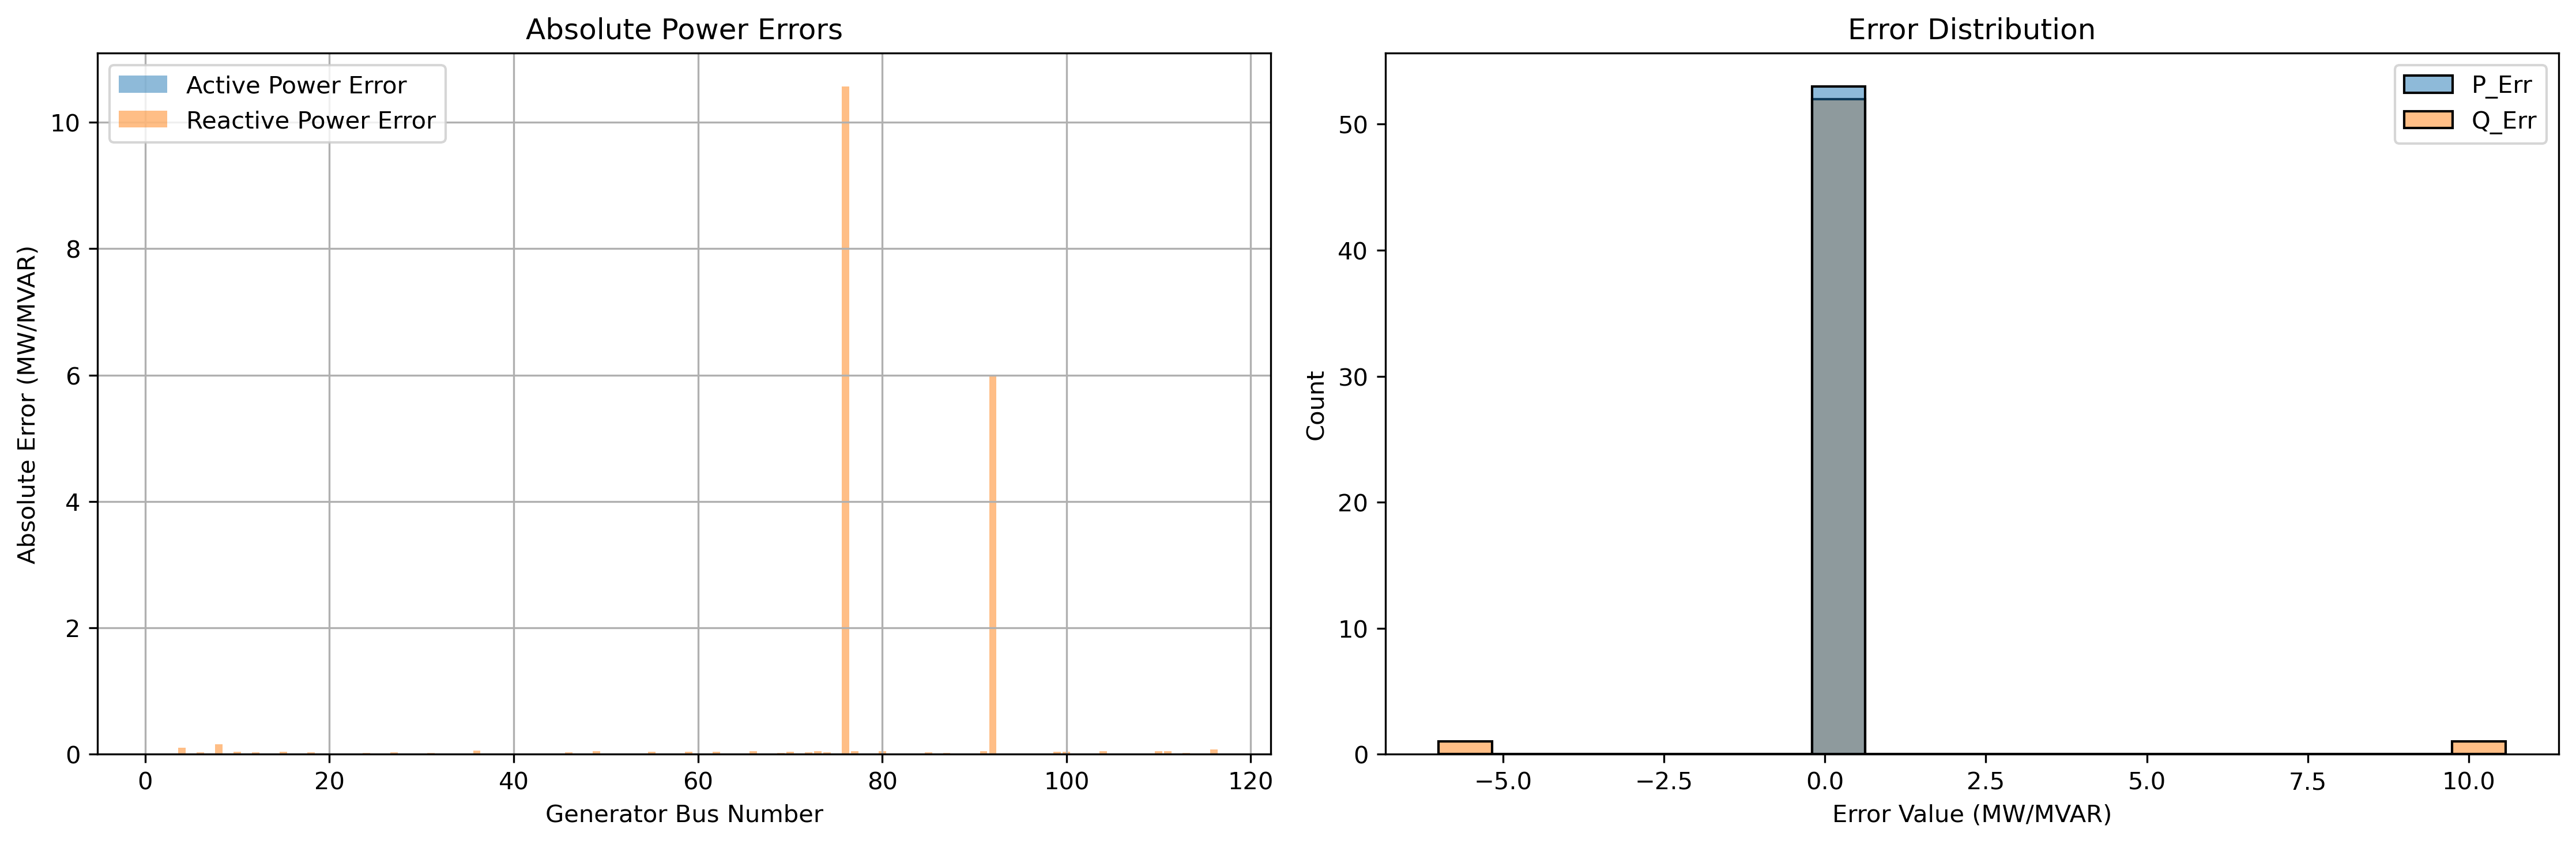
\includegraphics[width=\textwidth]{error_analysis.png}
    \caption{Error Distribution and Magnitude Analysis}
    \label{fig:error_analysis}
\end{figure}

\subsection{Active Power Errors}
The comparison between original and DSS values for active power shows excellent agreement:
\begin{itemize}
    \item Average error: -0.000044 MW
    \item Maximum absolute error: 0.0023 MW
    \item Negligible discrepancies across all generators
\end{itemize}

\subsection{Reactive Power Errors}
Reactive power comparison shows generally good agreement with some notable exceptions:
\begin{itemize}
    \item Average error: 0.078 MVAR
    \item Maximum absolute error: 10.57 MVAR
    \item Most generators show errors below 1.0 MVAR
\end{itemize}

\section{Key Findings}
\begin{enumerate}
    \item The OpenDSS implementation shows excellent accuracy in active power calculations
    \item Reactive power calculations show good overall agreement with a few outliers
    \item The largest discrepancies appear in reactive power calculations for specific generators
    \item The system maintains power balance within acceptable tolerances
\end{enumerate}

\section{Recommendations}
\begin{enumerate}
    \item Review voltage control settings for generators with large reactive power discrepancies
    \item Verify transformer tap settings affecting reactive power flow
    \item Consider implementing more detailed generator models for improved accuracy
    \item Monitor generators with significant reactive power errors during dynamic simulations
\end{enumerate}

\section{Conclusion}
The analysis demonstrates that the OpenDSS implementation of the IEEE 118-bus system provides highly accurate results for active power flow calculations. While reactive power calculations show some discrepancies, the overall performance is satisfactory for power system analysis purposes. The identified discrepancies in reactive power calculations should be monitored but do not significantly impact the system's overall performance.

\end{document} 